\question Answer all of the questions
\begin{parts}
	\part You hold a negatively charged rod (rod 1) near a second rod (rod 2), which is suspended by an insulating thread, and find that the second rod is attracted to the first one. Which of the following are possible? (Check all that apply)
	\begin{todolist}
		\item Rod 2 is positively charged
		\item Rod 2 is negatively charged
		\item Rod 2 is neutral
	\end{todolist}
	\part In the diagram below, there is an electric field in the upward direction due to charges not shown. Which diagram best describes the charge distribution on a neutral metal block?
	\begin{figure}[ht!]
		\centering
		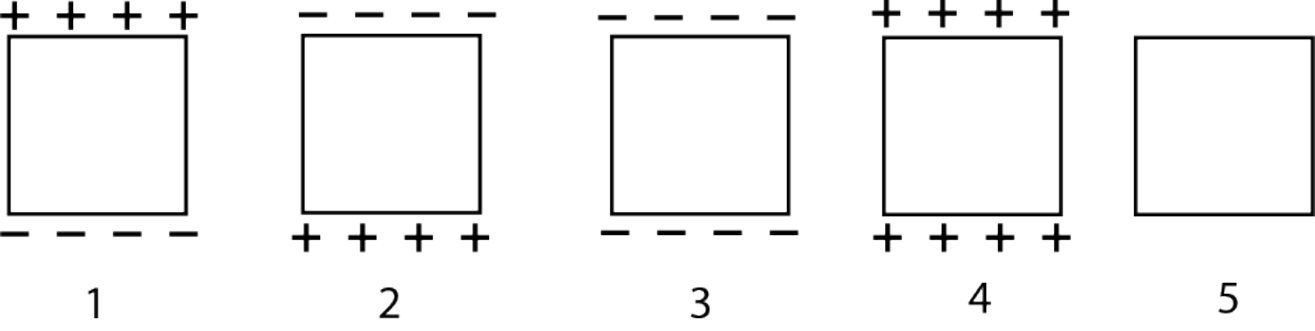
\includegraphics[width=8cm]{metal_block}
	\end{figure}
	\part Which of the following are true statements? (Check all that apply)
	\begin{todolist}
	\item In equilibrium, the average velocity of electrons $\bar{v}$ within a metal is 0
	\item The electric field inside of a metal is 0 under all circumstances
	\item Excess charge on an insulator cannot reside on the surface
	\item Conductors cannot be polarized
	\item In a metal any excess charge must be on the surface
	\end{todolist}
	
	\part Which is a better test of the existence and sign of the charge on an object, repulsion or attraction to a charged tape? Why? Explain briefly but clearly.
\end{parts}